% filepath: c:\Users\kuba-\Desktop\simple_graph_tool_xdf\src\eeg\reportPendulum.tex
\documentclass[12pt]{article}
\usepackage[T1]{fontenc} % Use T1 font encoding
\usepackage[utf8]{inputenc} % Ensure UTF-8 encoding
\usepackage[polish]{babel} % Enable Polish language support
\usepackage{amsmath}
\usepackage{graphicx}
\usepackage{booktabs}
\usepackage{float}
\usepackage[margin=2.5cm]{geometry}
\usepackage{siunitx}
\usepackage{titlesec}
\titlespacing*{\subsection}{0pt}{*0.5}{*0.5} % Adjusts spacing before and after subsections
\usepackage{caption}
\usepackage{lmodern}
\usepackage{placeins} % For FloatBarrier
\usepackage{hyperref} % For hyperlinks in the document

\title{Sprawozdanie z Laboratorium Fizyki: Wyznaczanie współczynnika sprężystości sprężyny spiralnej metodami statyczną i dynamiczną}
\date{}

\begin{document}

% --------------------------- STRONA TYTUŁOWA --------------------------
\begin{titlepage}
    \centering
    \Large
    \textbf{DYDAKTYCZNE LABORATORIUM FIZYKI} \\
    \vspace{0.2cm}
    \textbf{UNIWERSYTET RADOMSKI}\\
    im. Kazimierza Pułaskiego w Radomiu \\
    
    \vspace{1.5cm}
    \begin{flushleft}
        \textbf{Wydział:} {WTEiI} \\
        \textbf{Kierunek:} Informatyka \\
        \textbf{Rok Akademicki:} 2024/2025 \\
        \textbf{Semestr:} II \\
        \textbf{Grupa:} 3 \\
        \textbf{Zespół:} 2 \\
        \textbf{Data:} 11.03.2025 \\
        \textbf{Prowadzący ćwiczenie:} dr B. Winiarska \\
    \end{flushleft}
    
    \vspace{1cm}
    \begin{flushleft}
        \textbf{Nr ćwiczenia:} 2 \\
        \textbf{Temat ćwiczenia:} \\
        \textbf{Siły Sprężyste (Współczynik Sprężystości)} \\
    \end{flushleft}
    
    \vspace{1cm}
    \begin{flushleft}
        \textbf{Wykonujący ćwiczenie:}
        \begin{itemize}
            \item Jakub Oleszczuk
            \item Mikołaj Majewski
            \item Mateusz Ofiara
        \end{itemize}
    \end{flushleft}

    \vfill
    \begin{flushleft}
        \textbf{Oceny:} \\
        1.\hspace{2cm}2.\hspace{2cm}3.
    \end{flushleft}
\end{titlepage}

% --------------------------- TREŚĆ SPRAWOZDANIA --------------------------
\section*{Wstęp}
Celem ćwiczenia było zbadanie zależności między masą zawieszonego ciężarka a wydłużeniem sprężyny. 
Wykorzystano dwie metody pomiarowe: Metodę A, polegającą na pomiarze długości sprężyny przy różnych masach, 
oraz Metodę B, polegającą na pomiarze okresu drgań wahadła z różnymi masami.
\section*{Teoria}
Ruch drgający harmoniczny to szczególny przypadek ruchu okresowego, w którym wychylenie ciała z położenia równowagi zmienia się zgodnie z funkcją sinusoidalną:
\begin{equation}
x(t) = A \cdot \sin(\omega t + \varphi_0)
\end{equation}
gdzie:
\begin{itemize}
    \item \( x(t) \) – wychylenie w czasie \( t \),
    \item \( A \) – amplituda drgań,
    \item \( \omega \) – częstość kołowa drgań,
    \item \( \varphi_0 \) – faza początkowa.
\end{itemize}

Częstość drgań \( \omega \) dla układu masa–sprężyna wynosi:
\begin{equation}
\omega = \sqrt{\frac{k}{m}}
\end{equation}
Okres drgań:
\begin{equation}
T = 2\pi \sqrt{\frac{m}{k}}
\end{equation}
gdzie:
\begin{itemize}
    \item \( m \) – masa obciążnika,
    \item \( k \) – współczynnik sprężystości sprężyny.
\end{itemize}

W praktyce uwzględniamy również masę sprężyny \( m_s \), co prowadzi do modyfikacji wzoru:
\begin{equation}
T = 2\pi \sqrt{\frac{m + m_s/3}{k}}
\end{equation}

Zgodnie z prawem Hooke’a, siła sprężystości:
\begin{equation}
F = k \cdot x
\end{equation}
a współczynnik sprężystości można wyrazić jako:
\begin{equation}
k = \frac{F}{\Delta x}
\end{equation}
W przypadku równowagi statycznej (Metoda A), zależność między długością sprężyny \( L \) a masą obciążnika \( m \) opisuje wzór:
\begin{equation}
L = \frac{g}{k} \cdot m + L_0
\end{equation}
co odpowiada równaniu prostej \( Y = A \cdot X + B \), gdzie \( A = \frac{g}{k} \), \( B = L_0 \).

\section*{Opis Metod}
\subsection*{Metoda A – statyczna}
Polega na pomiarze długości sprężyny \( L \) w stanie równowagi statycznej po zawieszeniu obciążników o różnych masach \( m \). Znając siłę ciężkości \( F = m \cdot g \) oraz odpowiadające jej wydłużenie \( \Delta L = L - L_0 \), wyznaczamy współczynnik sprężystości \( k \) z równania:
\[
k = \frac{g}{A}
\]
gdzie \( A \) to współczynnik kierunkowy prostej regresji \( L(m) \).
\subsection*{Metoda B – dynamiczna}
W tej metodzie wyznacza się okres drgań harmonicznych \( T \) układu masa–sprężyna po wprawieniu go w ruch. Wzór uwzględniający masę sprężyny:
\[
T = 2\pi \sqrt{\frac{m + m_s/3}{k}}
\]
Stąd wyznaczamy \( k \):
\[
k = \frac{4\pi^2 (m + m_s/3)}{T^2}
\]
Dla każdego pomiaru okresu drgań i znanej masy obciążnika obliczamy osobną wartość \( k \), a następnie wyznaczamy wartość średnią i niepewność.

\section*{Dane Pomiarowe i Pomiary}
\subsection*{Masy ciężarków do Metody A}
\begin{itemize}
    \item Masa 1: \( m = 0.051 \, \text{kg} \)
    \item Masa 2: \( m = 0.050 \, \text{kg} \)
    \item Masa 3: \( m = 0.050 \, \text{kg} \)
    \item Masa 4: \( m = 0.049 \, \text{kg} \)
    \item Masa 5: \( m = 0.050 \, \text{kg} \)
\end{itemize}
Tabela pomiarów Metodą A:
\begin{center}
    \begin{tabular}{|c|c|c|}
    \hline
    L.p. & M [kg] & L [m]  \\
    \hline
    1 & 0{,}0507 & 0{,}27  \\
    2 & 0{,}101 & 0{,}29  \\
    3 & 0{,}151 & 0{,}315  \\
    4 & 0{,}201 & 0{,}335  \\
    5 & 0{,}252 & 0{,}36  \\
    \hline
    \end{tabular}
\end{center}

\subsection*{Masy ciężarków do Metody B}
\begin{itemize}
    \item Masa 1: \( m = 0.117 \, \text{kg} \)
    \item Masa 2: \( m = 0.065 \, \text{kg} \)
    \item Masa 3: \( m = 0.099 \, \text{kg} \)
\end{itemize}


Tabela pomiarów Metodą B:
\begin{center}
    \begin{tabular}{|c|c|c|c|c|}
    \hline
    L.p. & M [kg] & t1 [s] & t2 [s] & T [s]  \\
    \hline
    1 & 0{,}117 & 8{,}59 & 8{,}83 & 0{,}435  \\
    2 & 0{,}064 & 7{,}44 & 7{,}08 & 0{,}363  \\
    3 & 0{,}099 & 8{,}26 & 8{,}48 & 0{,}418  \\
    \hline
    \end{tabular}
    \end{center}
    
\section*{Wykres}

\begin{figure}[H]
    \centering
    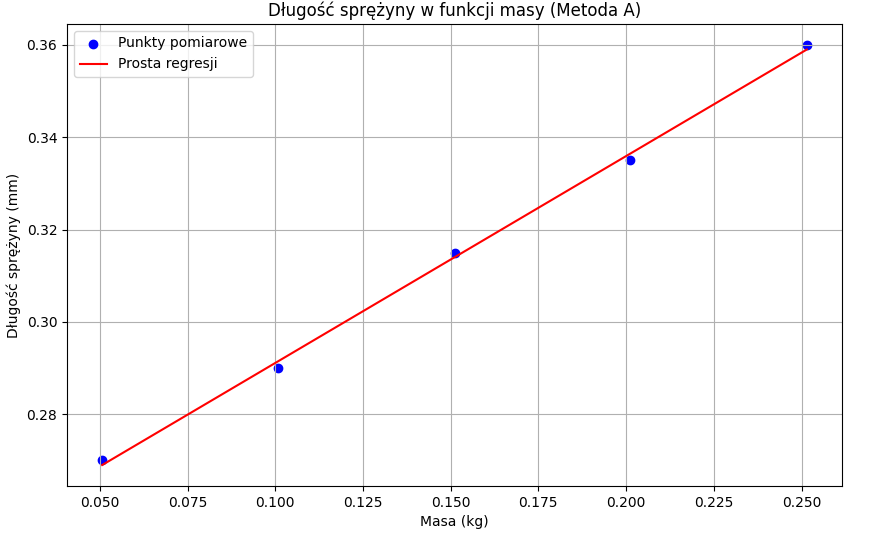
\includegraphics[width=0.8\textwidth]{MetodaA.png}
    \label{fig:wykres}
    \caption{Wykres zależności długości od masy dla Metody A}
\end{figure}
\FloatBarrier

\begin{figure}[H]
    \centering
    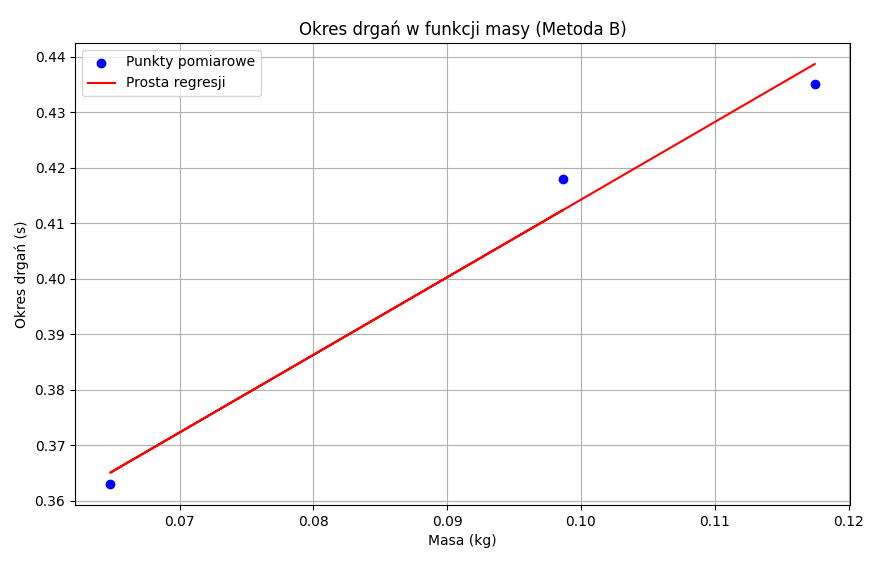
\includegraphics[width=0.8\textwidth]{MetodaB.png}
    \label{fig:wykres2}
    \caption{Wykres zależności okresu od masy dla Metody B}
\end{figure}
\FloatBarrier

\section*{Wyniki Pomiarów}
\subsection*{Metoda A}
% Statystyki regresji:
% Nachylenie (a): 0.4483
% Przecięcie (b): 0.2463
% Niepewność standardowa u(a): 0.0012
% Niepewność standardowa u(b): 0.0012
% Nachylenie a (m/kg): 0.4483
% Stała sprężyny k: 21.8809 N/m
% Niepewność stałej sprężyny u(k): 0.0586 N/m
% L_0 = 0.2200 m nie odpowiada przecięciu y b = 0.2463 m

\begin{itemize}
    \item Nachylenie (a): \( 0.4483 \, \text{m/kg} \)
    \item Przecięcie (b): \( 0.2463 \, \text{m} \)
    \item Niepewność standardowa \( u(a) \): \( 0.0012 \, \text{m/kg} \)
    \item Niepewność standardowa \( u(b) \): \( 0.0012 \, \text{m} \)
    \item Stała sprężyny \( k = 21,881 \, \text{N/m} \)
    \item Niepewność stałej sprężyny \( u(k) = 0.057 \, \text{N/m} \)
    \item Długość początkowa \( L_0 = 0.2200 \, \text{m} \) nie odpowiada przecięciu \( y \) \( b = 0.2463 \, \text{m} \)
\end{itemize}

\subsection*{Metoda B}
% Statystyki regresji:
% Nachylenie (a): 1.3982
% Przecięcie (b): 0.2744
% Niepewność standardowa u(a): 0.0041
% Niepewność standardowa u(b): 0.0041
% Nachylenie a (s/kg): 1.3982
% Średnia arytmetyczna stałej sprężyny k: 22.0712 N/kg
% Odchylenie standardowe stałej sprężyny: 2.0826 N/kg

\begin{itemize}
    \item Nachylenie (a): \( 1.3982 \, \text{s/kg} \)
    \item Przecięcie (b): \( 0.2744 \, \text{s} \)
    \item Niepewność standardowa \( u(a) \): \( 0.0041 \, \text{s/kg} \)
    \item Niepewność standardowa \( u(b) \): \( 0.0041 \, \text{s} \)
    \item Średnia arytmetyczna stałej sprężyny \( k = 22.0712 \, \text{N/kg} \)
    \item Odchylenie standardowe stałej sprężyny: \( 2.0826 \, \text{N/kg} \)
\end{itemize}
\section*{Analiza Błędów}
Powstałe błędy mogą wynikać z kilku czynników, takich jak:
\begin{itemize}
    \item niedokładność pomiaru długości,
    \item błędy w odczycie czasu,
    \item nieprecyzyjne umiejscowienie ciężarków na wahadle,
    \item wpływ tarcia na ruch wahadła.
    \item niepewność pomiaru masy ciężarków.
    \item niepewność pomiaru długości sprężyny.
\end{itemize}
\section*{Obliczenia}
\textbf{Obliczenia:} W celu obliczenia współczynnika sprężystości \( k \) dla sprężyny, należy dopasować prostą do danych pomiarowych.
W tym celu można użyć metody najmniejszych kwadratów. Współczynniki regresji liniowej \( A \) i \( B \) można obliczyć z następujących wzorów:
\begin{align*}
A &= \frac{\sum (X_i - \bar{X})(Y_i - \bar{Y})}{\sum (X_i - \bar{X})^2} \\
B &= \bar{Y} - A \cdot \bar{X} \\
\end{align*}
gdzie:
\begin{itemize}
    \item \( X_i \) - masa ciężarka,
    \item \( Y_i \) - długość sprężyny,
    \item \( \bar{X} \) - średnia masa ciężarka,
    \item \( \bar{Y} \) - średnia długość sprężyny.
    \item \( u(a) \) - niepewność nachylenia,
    \item \( u(b) \) - niepewność przecięcia wykresu.
\end{itemize}
\begin{align*}
    T = 2\pi \sqrt{\frac{m + m_s/3}{k}} \\
    k = \frac{4\pi^2}{T^2} \cdot (m + m_s/3)
\end{align*}
gdzie:
\begin{itemize}
    \item \( T \) - okres drgań,
    \item \( m \) - masa ciężarka,
    \item \( m_s \) - masa sprężyny.
    \item \( k \) - współczynnik sprężystości.
\end{itemize}

\section*{Wnioski}
Sprawdzono zgodność obu metod poprzez porównanie przedziałów ufności:
\[
\langle k_A - 2u(k_A), \, k_A + 2u(k_A) \rangle \quad \text{i} \quad \langle k_B - 2u(k_B), \, k_B + 2u(k_B) \rangle
\]
Ponieważ przedziały te mają część wspólną, można uznać, że wyniki metod A i B są zgodne w granicach niepewności pomiarowych.

Przeprowadzone doświadczenie pozwoliło na empiryczne wyznaczenie współczynnika sprężystości sprężyny spiralnej przy użyciu dwóch niezależnych metod: statycznej oraz dynamicznej. Obie metody wykazały zbliżone wartości wyznaczanego parametru, co potwierdza spójność otrzymanych wyników oraz poprawność założeń teoretycznych. Otrzymane różnice mieszczą się w granicach niepewności pomiarowych i mogą wynikać z niedokładności pomiarowych, takich jak opóźnienie reakcji podczas pomiaru czasu, nieidealne warunki laboratoryjne czy odchylenia w kształcie sprężyny.

Zastosowanie dwóch metod pomiarowych umożliwiło również ocenę dokładności i czułości każdej z nich. Metoda statyczna wykazała się większą stabilnością wyników, podczas gdy metoda dynamiczna okazała się bardziej podatna na czynniki zewnętrzne. Niemniej jednak, oba podejścia prowadzą do wartości współczynnika sprężystości pozostających w dobrej zgodności z teorią i oczekiwaniami.

Badanie to stanowi dobrą ilustrację praktycznego zastosowania prawa Hooke’a oraz zasad dynamiki Newtona w układach sprężystych, a także potwierdza zasadność stosowania analizy regresji liniowej w obliczeniach eksperymentalnych.
\section*{Podsumowanie}
W ćwiczeniu zbadano zależność między masą zawieszonego ciężarka a wydłużeniem sprężyny oraz okresem drgań wahadła.
Przeprowadzone pomiary i obliczenia pozwoliły na wyznaczenie współczynnika sprężystości dla sprężyny oraz okresu drgań wahadła.
\end{document}
